\begin{figure}[!t]
  \centering
  \setlength{\tabcolsep}{0.5pt} % adjust spacing between images
  \renewcommand{\arraystretch}{0.4}

  % Add a border using \fbox around the tabular
  \begin{center}
    \fbox{%
      \begin{tabular}{c c c}
        \textbf{Grad-CAM} & \textbf{Layer-CAM} & \textbf{Grad-CAM++} \\
        [2pt]
        % First row of images
        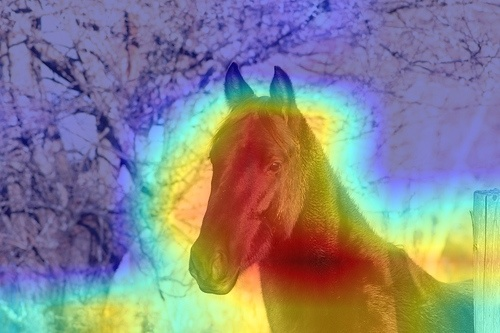
\includegraphics[width=0.18\linewidth, height=0.18\linewidth]{figures/cams/gradcam/2007_009807_12} &
        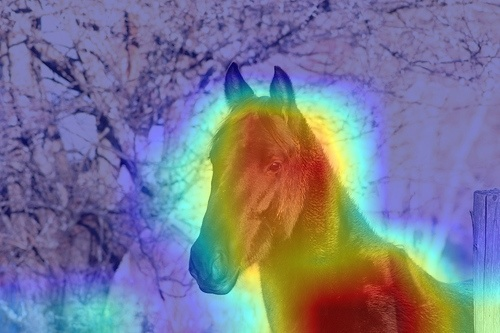
\includegraphics[width=0.18\linewidth, height=0.18\linewidth]{figures/cams/layercam/2007_009807_12} &
        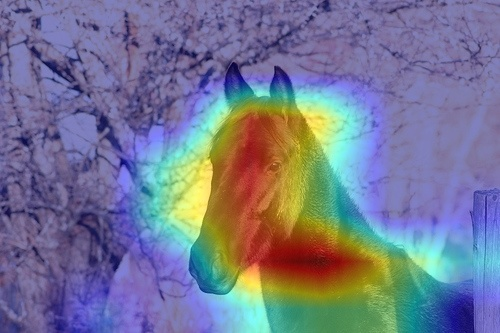
\includegraphics[width=0.18\linewidth, height=0.18\linewidth]{figures/cams/gradcampp/2007_009807_12} \\

        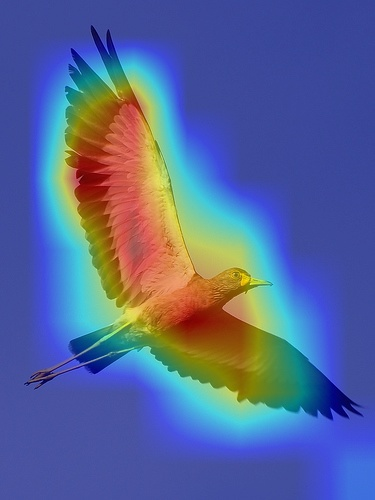
\includegraphics[width=0.18\linewidth, height=0.18\linewidth]{figures/cams/gradcam/2011_001967_2} &
        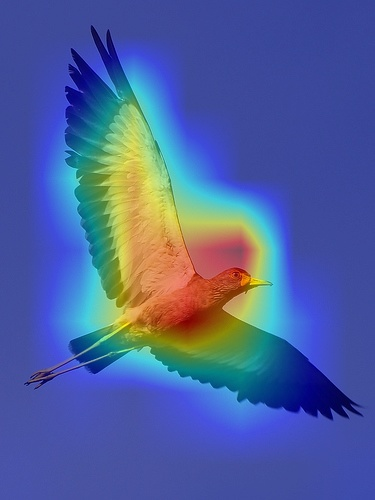
\includegraphics[width=0.18\linewidth, height=0.18\linewidth]{figures/cams/layercam/2011_001967_2} &
        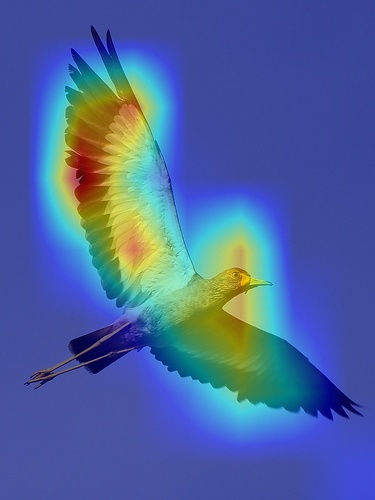
\includegraphics[width=0.18\linewidth, height=0.18\linewidth]{figures/cams/gradcampp/2011_001967_2} \\

        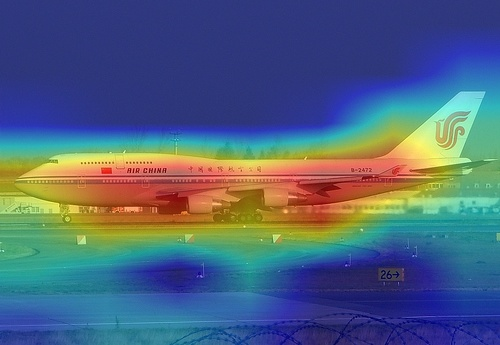
\includegraphics[width=0.18\linewidth, height=0.18\linewidth]{figures/cams/gradcam/2008_003976_0} &
        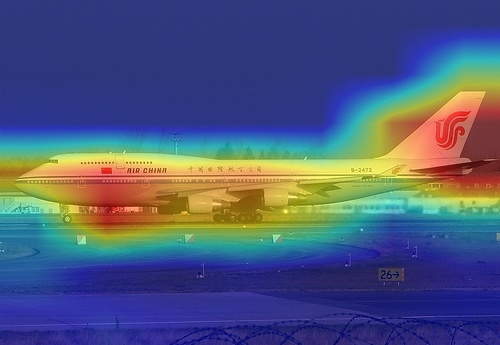
\includegraphics[width=0.18\linewidth, height=0.18\linewidth]{figures/cams/layercam/2008_003976_0} &
        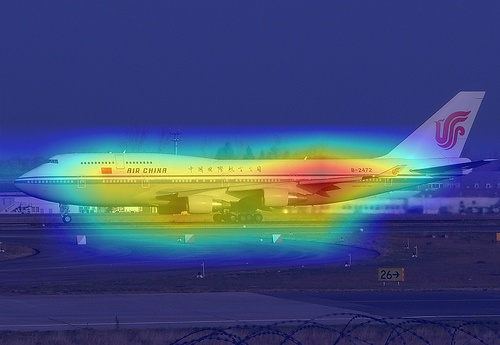
\includegraphics[width=0.18\linewidth, height=0.18\linewidth]{figures/cams/gradcampp/2008_003976_0} \\

      \end{tabular}
    }
  \end{center}

  \caption{Comparison of CAM visualization methods on the Pascal VOC dataset for single class scenario. Columns show Grad-CAM, Layer-CAM, and Grad-CAM++ respectively. Each row corresponds to a different example image.}
  \label{fig:cam_variation_singleclass}
\end{figure}


\section{Strengths of the Approach}
\label{sec:strengths_of_approach}

The proposed UniCL-AffSeg framework offers several notable strengths that position it as a promising advancement in weakly supervised semantic segmentation (WSSS). By integrating the UniCL framework with a Swin Transformer backbone and affinity-based refinement strategies, the approach leverages multi-modal learning, hierarchical feature extraction, and semantic consistency to overcome common limitations in WSSS pipelines. The following subsections outline these key strengths.

\subsection{Multi-Modal Learning and Unified Objectives}
UniCL's unified contrastive and classification objectives enable robust alignment between image and text modalities, enhancing feature representations without requiring dense annotations. This multi-modal synergy facilitates better image-text correspondence, leading to more discriminative class activation maps (CAMs) compared to traditional single-modal methods. As a result, the framework can generalize across diverse datasets and handle complex scenes with multiple objects, reducing reliance on external cues like saliency maps.

\subsection{Hierarchical Feature Extraction with Swin Transformer}
The Swin Transformer's hierarchical architecture provides multi-scale feature maps that capture both local details and global context, making it particularly suited for dense prediction tasks like segmentation. Unlike global attention mechanisms in ViT-based models, Swin's shifted-window design ensures computational efficiency while preserving fine-grained local information, such as object boundaries and textures. This locality bias improves boundary precision in CAMs, addressing a common weakness in WSSS where activations often miss intricate object parts.

\subsection{Affinity-Based Refinement for Semantic Consistency}
The affinity-based CAM refinement technique, which combines encoder-derived affinity maps with decoder affinities, promotes semantic coherence by propagating information across pixel regions. This approach mitigates noise and fragmentation in initial CAMs, leading to more reliable pseudo-labels. By selecting high-quality affinity maps through deviation scoring, the method ensures stability and reduces overfitting, resulting in improved segmentation quality without additional supervision.

\subsection{Efficiency and Scalability}
The overall framework is computationally efficient, benefiting from Swin's linear complexity and UniCL's pre-trained multi-modal representations. This allows for scalable training on large datasets like PASCAL VOC 2012, making the approach feasible for real-world applications with limited resources. Furthermore, the integration of Pixel-Adaptive Refinement (PAR) enhances boundary accuracy by incorporating color and spatial similarities, providing a lightweight yet effective post-processing step.

In summary, these strengths collectively enable UniCL-AffSeg to generate higher-quality CAMs and pseudo-labels, narrowing the gap between weakly supervised and fully supervised segmentation while maintaining practicality. Future iterations could build on these advantages to further optimize performance in challenging scenarios.